\section{AIIDE: Artificial Intelligence and Interactive Digital Entertainment}\label{subsecAIIDE}

The AIIDE Starcraft AI Competition is the longest running annual Starcraft competition, and has been held every year since 2010 along with the AAAI Artificial Intelligence and Interactive Digital Entertainment conference. Unlike the CIG and SSCAIT competitions, the AIIDE competition requires that all bots be open source, and that their source code will be published for public download after the competition has finished. Running 24 hours a day for 2 weeks with games played at super-human speed, the competition is a single round-robin format with the winner being the bot with the highest win percentage when the time limit has been reached. 

\subsection*{AIIDE 2016-17 Updates \& News}\label{subsecAIIDEnews}

The 2016 AIIDE competition had a total of 21 competitors, and the round robin games ran on 12 machines for nearly two weeks. A total of 90 round robin rounds were completed, with each bot playing 1800 games. No new rules or maps were used for the 2016 tournament that were not in place for the 2015 tournament. As the AIIDE competition was held shortly after the CIG competition, many of the submissions were the same, which is reflected in the results of both competitions. The top four finishers can be seen in Figure \ref{figAIIDEresults}, with Iron placing 1st, ZZZKbot placing 2nd, and tscmoo coming in 3rd place.

\vskip 2mm
\begin{figure}[h]
  \centering
  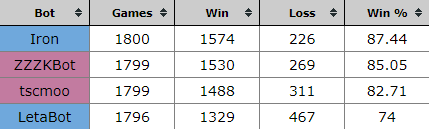
\includegraphics[width=1\columnwidth]{fig/aiide2016.png}
  \caption{Results of the top 4 finishers in the 2016 AIIDE competition. Iron and LetaBot are Terran bots, while ZZZBot and tscmoo played as Zerg.}
  \label{figAIIDEresults}
\end{figure}

In 2016, the AIIDE competition website was updated to include an archive\footnote{\url{http://www.cs.mun.ca/~dchurchill/starcraftaicomp/archive.shtml}} of data and results of all of the annual AIIDE and CIG competitions, including final results, bot source code and binary download links, and information about each bot. 

The 2017 AIIDE competition will have several updates:

\begin{itemize}
\item An updated map pool consisting of 10 new maps.
\item Updated tournament managing software capable of playing more games in the same period of time.
\item Support for BWAPI version 4.2.0
\item Bots that achieved a 30\% or higher win rate in the 2016 competition will be carried forward to 2017
\item Plans to support GPU computation for bots
\end{itemize}

\vskip 6mm